\documentclass{standalone}
%% Show/hide steps for standalone work — edit this line:
\makeatletter\AtBeginDocument{\@buildstepset{1,2,3,4,5,6,7,8,9,10}}\makeatother
\usepackage{tikz}
\usepackage{hsbcommon}
\begin{document}
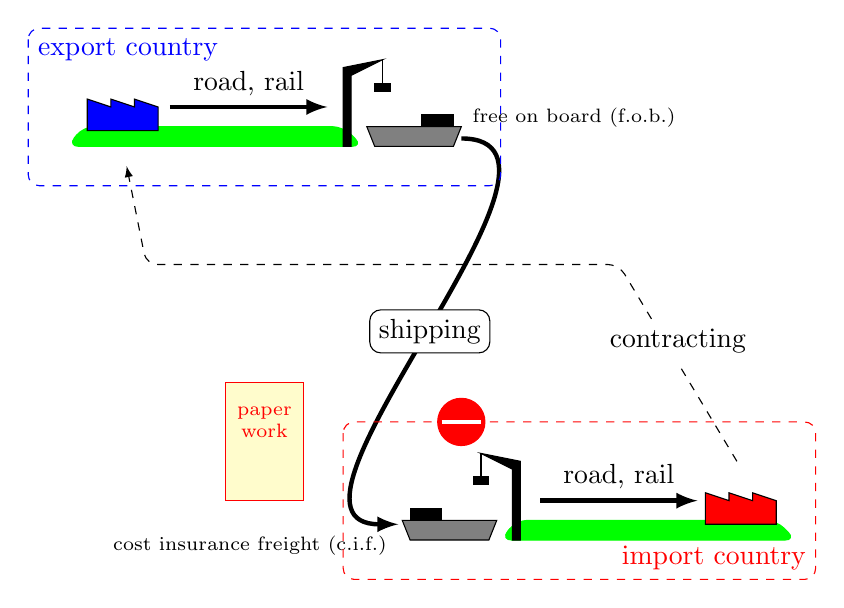
\begin{tikzpicture}
    \tikzset{
    myhouse/.pic={
        },
    myland/.pic={
        \filldraw[green,rounded corners] (0,0) -- (0.2,0.25) --  (3.5,0.25) -- (3.75,0) -- cycle;
        },
    myhouse/.pic={
        \filldraw (0,0.2) -- 
        (0,  0.6) -- (0.3,0.5) -- 
        (0.3,0.6) -- (0.6,  0.5) -- 
        (0.6,  0.6) -- (0.9,0.5) -- 
        (0.9,0.2) -- cycle;     
        },
    myhome/.pic={
        \filldraw (0,0) rectangle (0.5,0.4);
        \filldraw (-0.1,0.4) -- (0.25,0.75) -- (0.6,0.4) -- cycle;
        \filldraw[white,draw=black] (0.12,0) rectangle (0.22,0.25);
        \filldraw[white,draw=black] (0.3,0.1) rectangle (0.4,0.25);
    
        },
    myport/.pic={
        \draw[fill=black] (1.5,0) -- (1.5,1) -- (2,1.1) -- (1.6,0.9) -- (1.6,0) -- cycle;
        \draw (2,1.1) -- (2,0.8); \draw[fill=black] (1.9,0.8) rectangle (2.1,0.7);
        \draw[fill=gray] (1.9,0) -- (1.8,0.25) -- (3,0.25) -- (2.9,0) -- cycle;
        \draw[fill=gray!506] (2.5,0.25) rectangle (2.9,0.4);
        },
    mydocs/.pic={
        \draw[fill=yellow!20] (-0.5,0) 
        rectangle
        (0.5,-1.5);
        \node at (0,-0.5) {\parbox{1cm}{
                \centering
                \scriptsize
                paper\\ work
            }};
        },
    mydouane/.pic={
        \filldraw[red] (0,0) circle (0.3);
        \draw [ultra thick, white] (-0.25,0) -- (0.25,0);
    }
    }

    %%% draw the two countries

    \begin{scope}[fill=blue]
        \pic at (0,0) {myland};
        \pic at (0.25,0) {myhouse};
        \pic at (2,0) {myport};
        \ifstep{2}{\draw[->,>=latex,ultra thick] (1.3,0.5) -- node[above] {road, rail} (3.3,0.5);}
    \end{scope}

        
    \begin{scope}[fill=red,xshift=5cm,yshift=-5cm]
        \pic at (0.5,0) {myland} node (2) {};
        \pic at (3.1,0) {myhouse};
        \pic[xscale=-1] at (2.25,0) {myport};
        \ifstep{2}{\draw[->,>=latex,ultra thick] (1,0.5) -- node[above] {road, rail} (3,0.5);}
    \end{scope}

    %%% order
    \ifstep{1}{\draw[->,>=latex,dashed,rounded corners] (8.5,-4) to node[above,fill=white] {contracting} (7,-1.5) to  (1,-1.5) to (0.75,-0.25);}

    %%%
    \ifstep{3}{
        \draw[->,>=latex,ultra thick] (5,0.1)  node[above right] {\scriptsize free on board (f.o.b.)} to[out=0,in=180] node[fill=white,draw,thin,rounded corners] {shipping} (4.2,-4.8) node[below left] {\scriptsize cost insurance freight (c.i.f.)};
    }

    \ifstep{4}{
        \begin{scope}[color=red]
            \draw[dashed,rounded corners,blue] (-0.5,1.5) node[below right] {export country} rectangle (5.5,-0.5);
            \draw[dashed,rounded corners,red] (3.5,-3.5) rectangle (9.5,-5.5) node[above left] {import country};
            \draw (2.5,-3) pic {mydocs};
            \draw (5,-3.5) pic {mydouane};
        \end{scope}
    }

\end{tikzpicture}
\end{document}